\documentclass{report}
\usepackage{graphicx}
\usepackage{authblk}
\usepackage{amsmath}
\usepackage{listings}
\usepackage{subfigure}
\usepackage{algorithm2e}


\title{ME489 HW2}

\author{Ata Bora Çakmakci}
\author{Mustafa Yiğit Görgün}
\affil{Middle East Technical University}
\date{19 November 2023}

\begin{document}
\maketitle
\tableofcontents

\chapter{Introduction}
In this study, we developed an explicit in-time solver written in C language that uses the finite difference method to solve the linear advection equation given below.

\begin{equation}
\frac{\partial q}{\partial t} + \nabla \cdot(\mathbf{u} q) = 0
\end{equation}

The program we developed receives text from the user as a DAT file. It pulls user preferences, such as the number of nodes in the x and y directions, from the file it receives. It then creates nodes and mesh considering these preferences. Then nodes and neighbors are numbered using a linear index. And the initial conditions for those nodes are determined. Then, it finds the gradient using the first-order finite difference method, and then, using the fourth-order five-stage Runge-Kutta method, it integrates the resulting ordinary differential equation in time. Then it outputs the results in CSV format. The processed version of the test function and result is presented during the report.

\chapter{Code}
\section{"readInputFile" function}
This function accepts input as "filename" and "tag" and returns the value associated with the determined "tag" from the "filename.dat" file. The functions searches for the index of the "[" terms and if the index is zero the function starts reading the string. The function compares the string character by character with the tag and if the two match, the function reads the next line as a double and return the value.
\section{"RHSQ" function}
In this function, we completed first-order finite difference vs time-stepping operations. The finite difference technique consists of the following steps:

\begin{enumerate}
    \item Creating boundary conditions and reaching them.
    \item Calculating initial values for each point according to boundary conditions.
    \item Calculating the gradient for each node one by one with the formula below:
    \begin{align}
\left.\frac{\partial(v q)}{\partial y}\right|_{(i, j)} &\approx 
\begin{cases}
    \frac{v(i, j) q(i, j) - v(i, j-1) q(i, j-1)}{y(i, j) - y(i, j-1)} & \text{for } v(i, j) \geq 0 \\
    \frac{v(i, j+1) q(i, j+1) - v(i, j) q(i, j)}{y(i, j+1) - y(i, j)} & \text{for } v(i, j) < 0
\end{cases}
\end{align}
and 
\begin{align}
\left.\frac{\partial(v q)}{\partial y}\right|_{(i, j)} \approx 
\begin{cases}\frac{v(i, j) q(i, j)-v(i, j-1) q(i, j-1)}{y(i, j)-y(i, j-1)} & \text { for } v(i, j) \geq 0 \\ \frac{v(i, j+1) q(i, j+1)-u(i, j) q(i, j)}{y(i, j+1)-y(i, j)} & \text { for } v(i, j)<0\end{cases}
\end{align}
While calculating this point we use for loops the reach all nodes and when we reach this nodes we use if else to check the formula which we be going to use.And execute that formula. After that it stores all the data after the corresponding pointer with corresponding code:
 \pagebreak
  \begin{lstlisting}[language=C, caption={Gradient calculations}, label={yourlabel}]
mesh_t *msh = &solver->msh;
double DuqDx;
double DvqDy;
double *u = solver->u;
double *q = solver->q;
double *x = msh->x;
double *y = msh->y;
for(int j=0; j<msh->NY; j++){
for(int i=0; i<msh->NX; i++){
      
int n = j * msh->NX + i;
int m = n + msh->Nnodes;
if (u[n]>=0){
DuqDx=( u[n] * q[n] - u[msh->N2N[4*n]] 
* q[msh->N2N[4*n]] )/ (  x[n] - x[msh->N2N[4*n]] );
}else{ 
DuqDx=(-u[n]*q[n]+u[msh->N2N[4*n+2]]
* q[msh->N2N[4*n+2]]) / ( -x[n] + x[msh->N2N[4*n+2]] );
}
if (u[m]>=0){
DvqDy=(u[m]*q[n]-u[msh->N2N[4*n+3]+msh->Nnodes]
*q[msh->N2N[4*n+3]])/( y[n] - y[msh->N2N[4*n+3]] );
}else{ 
DvqDy=(-u[m]*q[n]+u[msh->N2N[4*n+1]+msh->Nnodes]
*q[msh->N2N[4*n+1]])/( -y[n] + y[msh->N2N[4*n+1]] );
}
}
\end{lstlisting}
 \item After we get gradient data at that time instance we will integrate over the time  our q values with given equation:

$$
\left.\frac{d q}{d t}\right|_{(i, j)}=\operatorname{rhs}(q)=-\left(\left.\frac{\partial(u q)}{\partial x}\right|_{(i, j)}+\left.\frac{\partial(v q)}{\partial y}\right|_{(i, j)}\right)
$$
and as a code:
\begin{verbatim}
double rhsq=-(DuqDx+DvqDy);
tstep->resq[n] = tstep->rk4a[stage] * tstep->resq[n] + tstep->dt * rhsq;
solver->q[n] = solver->q[n] + tstep->rk4b[stage] * tstep->resq[n];
\end{verbatim}
\end{enumerate}
\pagebreak
\section{"initialCondition" function}
At this section we define the initial condition to test function such as q, u and v function which we going to use in testing our function. And also calculate the initial values of each nodes with that function. We define our initial conditions as instructed in the homework instructions as following:
\begin{algorithm}
\For{$j=0$ \KwTo $msh->NY$}{
  \For{$i=0$ \KwTo $msh->NX$}{
    $x_c = 0.5$ \;
    $y_c = 0.75$ \;
    $r = 0.15$ \;
    $n = msh->NX \cdot j + i$ \;
    $solver->u[n] = \sin\left((0.5 + msh->x[n]) \cdot \pi \cdot 4\right) \cdot \sin\left((0.5 + msh->y[n]) \cdot \pi \cdot 4\right)$ \;
    $solver->u[n + msh->Nnodes] = \cos\left((0.5 + msh->y[n]) \cdot \pi \cdot 4\right) \cdot \cos\left((0.5 + msh->x[n]) \cdot \pi \cdot 4\right)$ \;
    $solver->q[n] = \sqrt{\left(msh->x[n] - x_c\right)^2 + \left(msh->y[n] - y_c\right)^2} - r$ \;
  }
}
\end{algorithm}
\chapter{Results}
The output of the program is a CSV type file. CSV type files stores the data by separating the data with commas. It is a type of file to tabulate the data. To post-process the results we used ParaView. We first imported the output files then we used ParaView's "TabletoPoint" feature to visualize our data. We did this in two ways in order to visualize our solution in two different ways. Firstly we selected the Z values as the Q values to have a rough understanding of what our solution becomes throughout the time steps. We then used "Delaunay2D" in order to interpolate between the points to form a surface. The results of the gradual formation of the solution can be seen in the Figure 3.1
\begin{figure}[htb]
\begin{center}
\subfigure[]{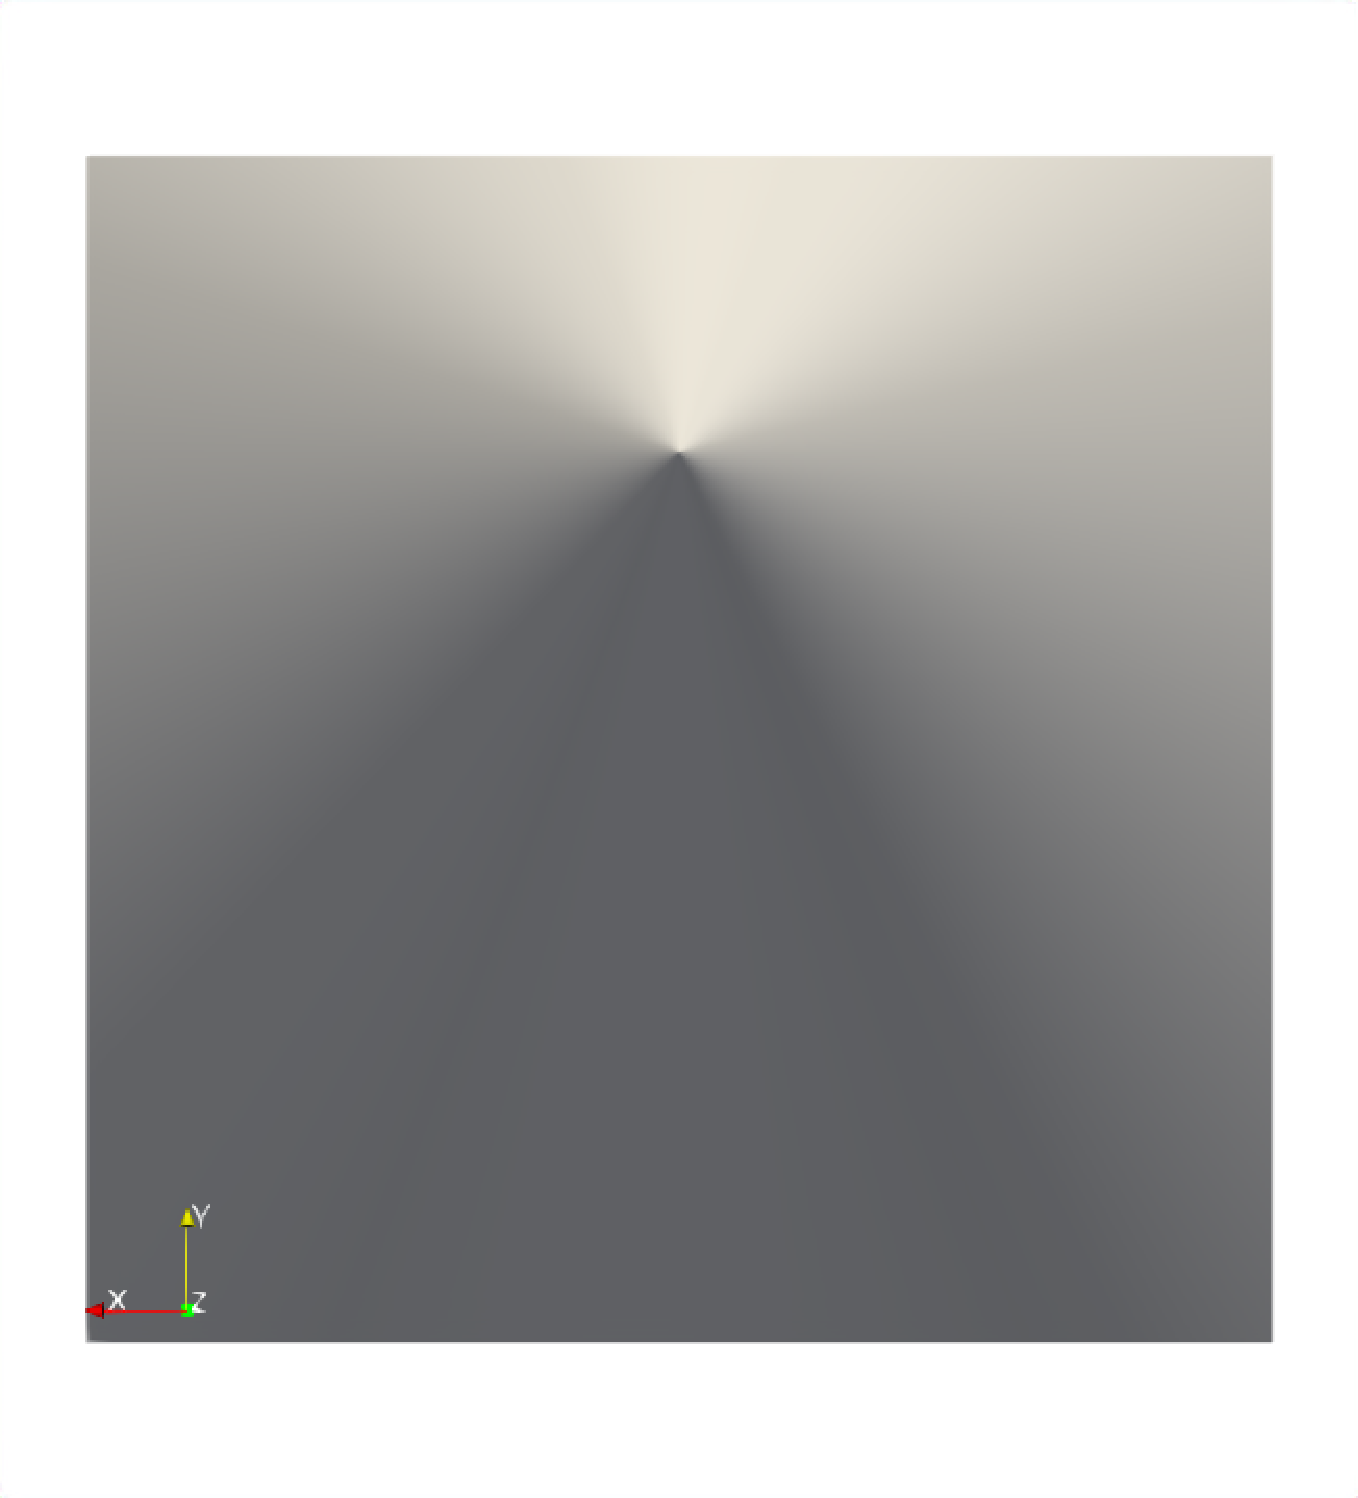
\includegraphics[height=1.1in,width=1.1in,angle=0]{scenes/scene_0.pdf}}
\subfigure[]{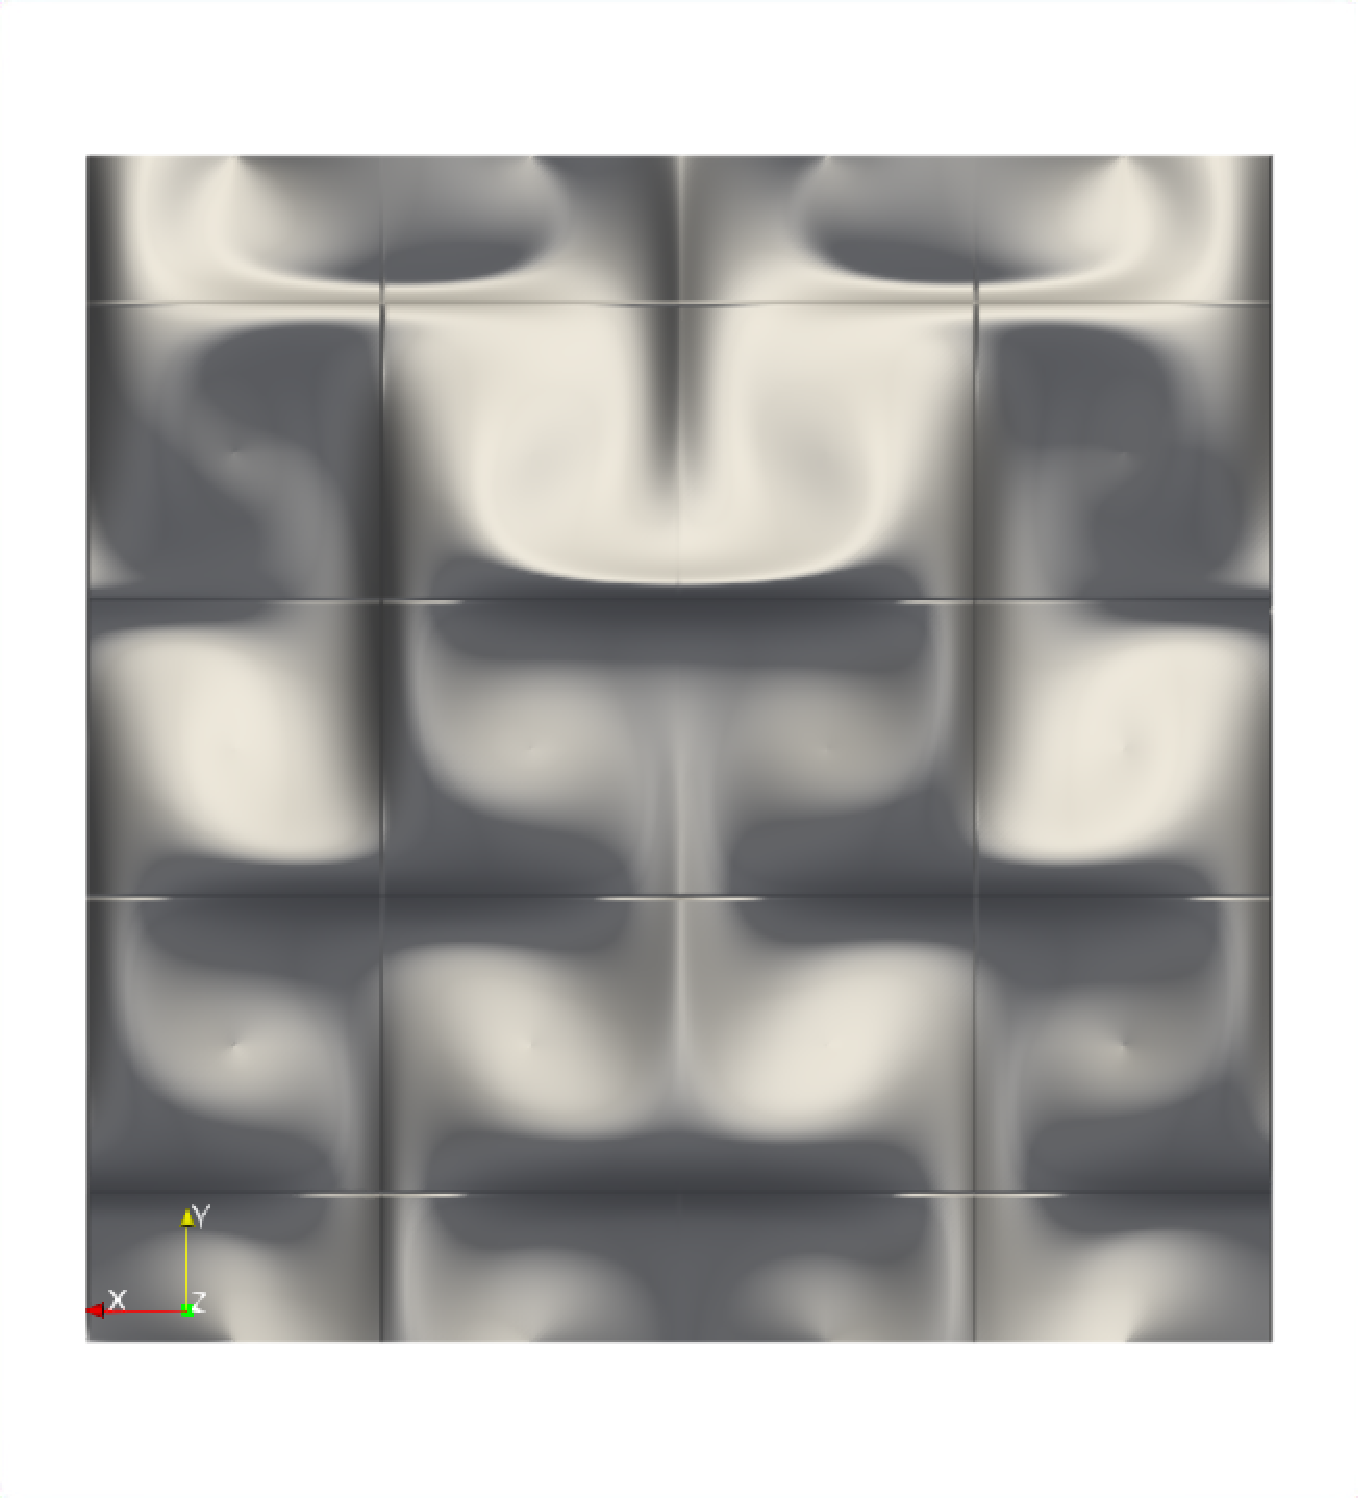
\includegraphics[height=1.1in,width=1.1in,angle=0]{scenes/scene_20.pdf}}
\subfigure[]{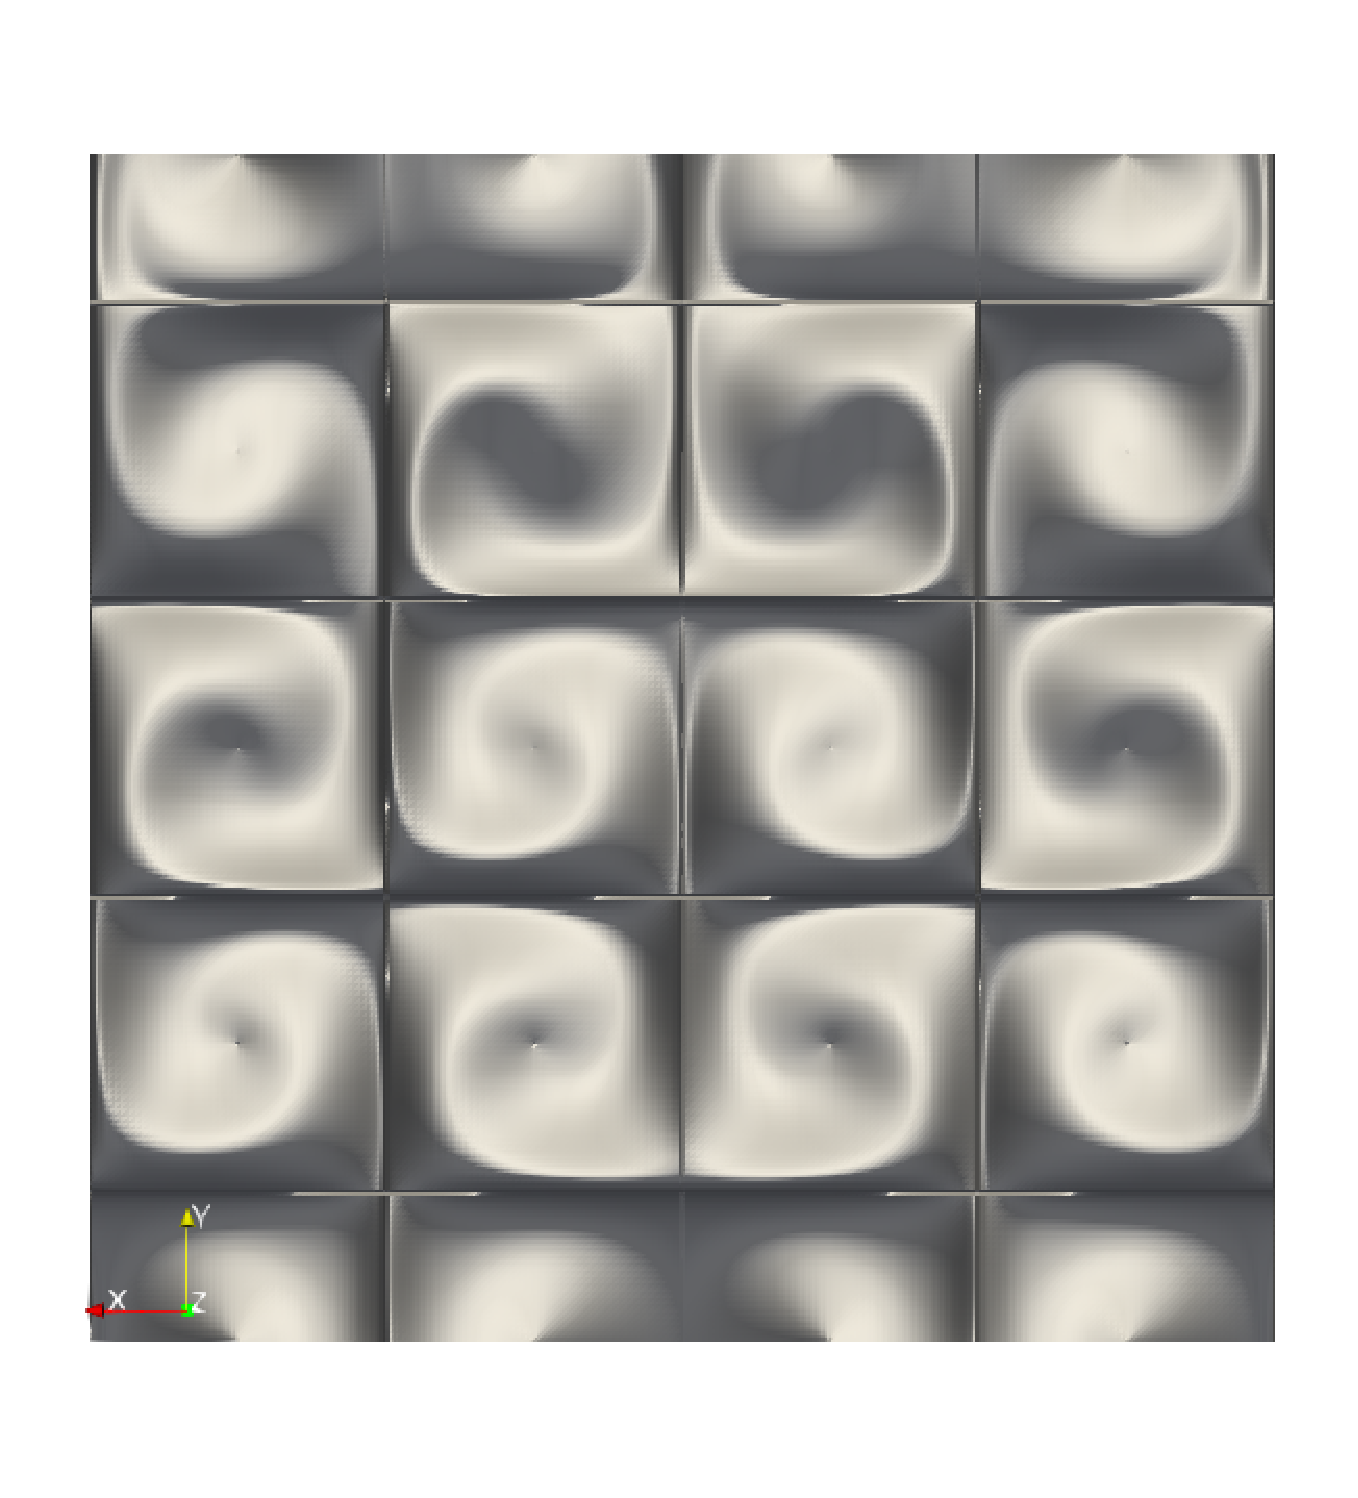
\includegraphics[height=1.1in,width=1.1in,angle=0]{scenes/scene_40.pdf}}
\subfigure[]{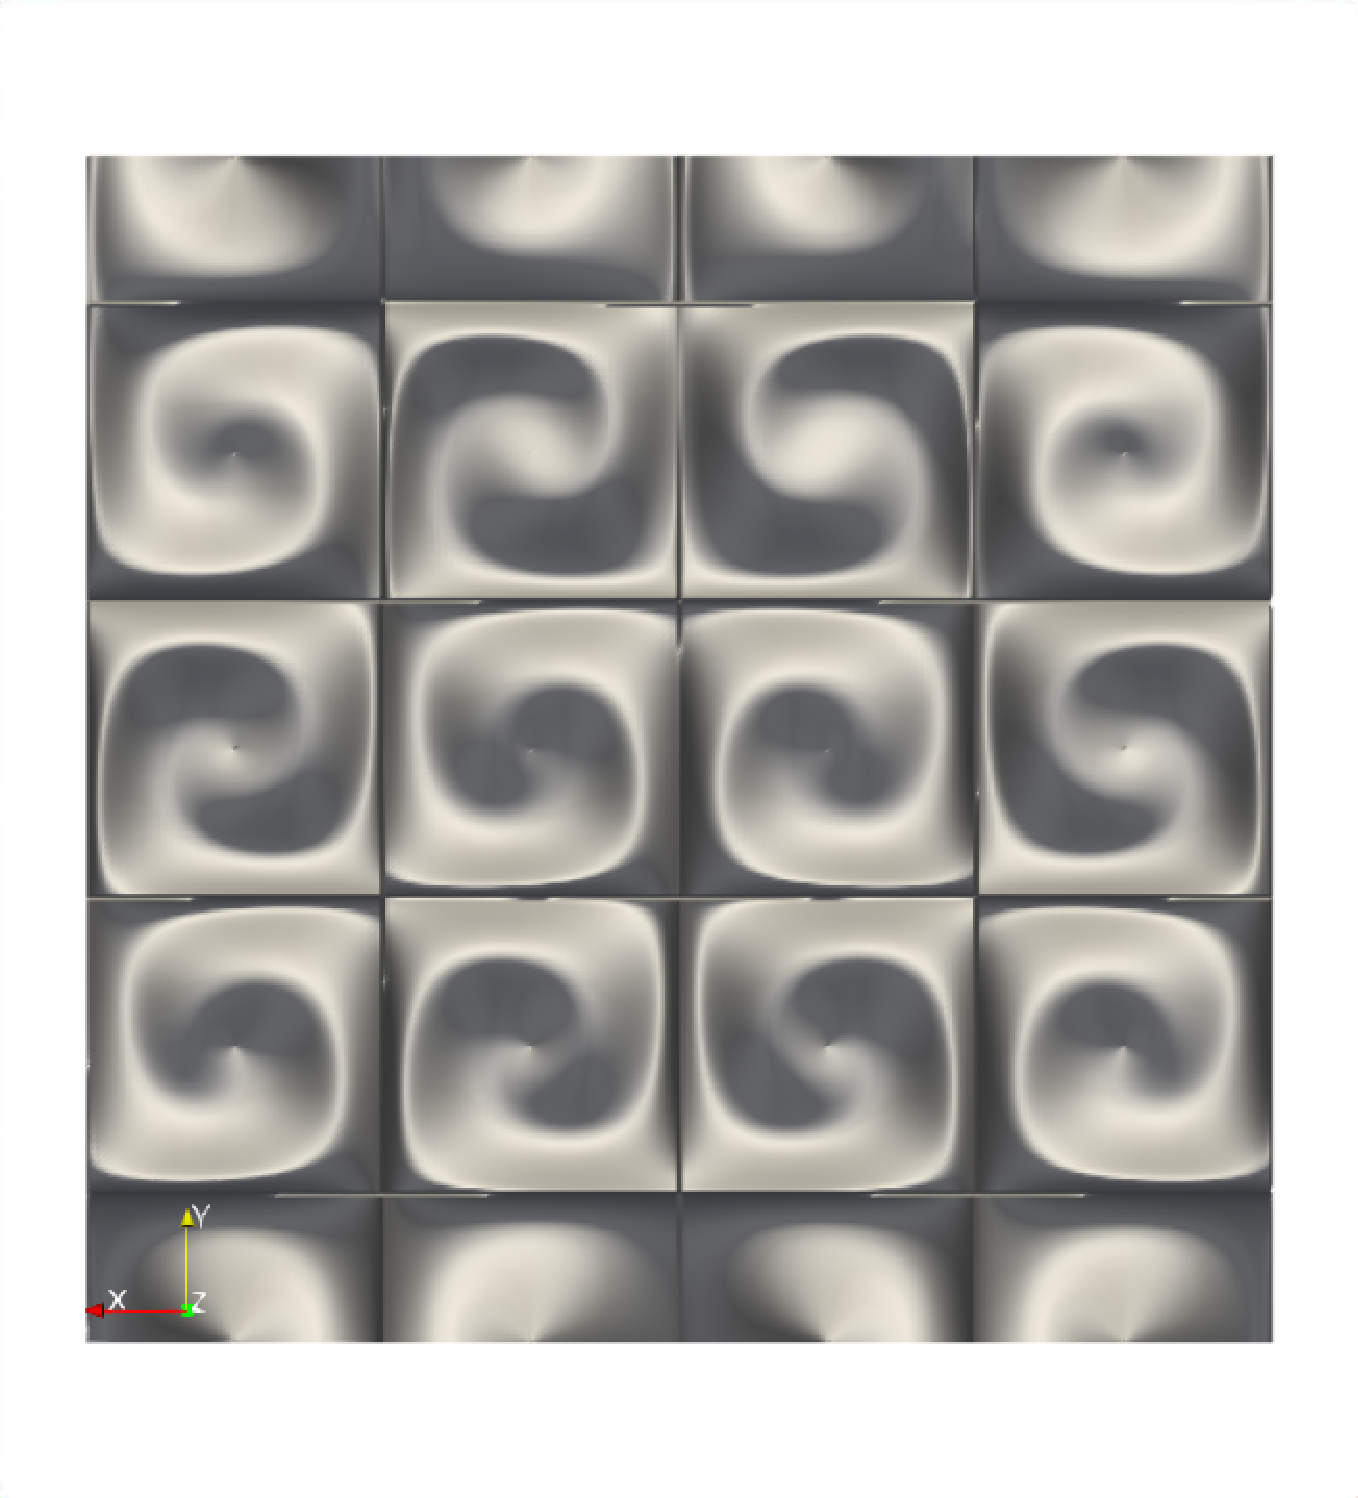
\includegraphics[height=1.1in,width=1.1in,angle=0]{scenes/scene_60.pdf}}
\subfigure[]{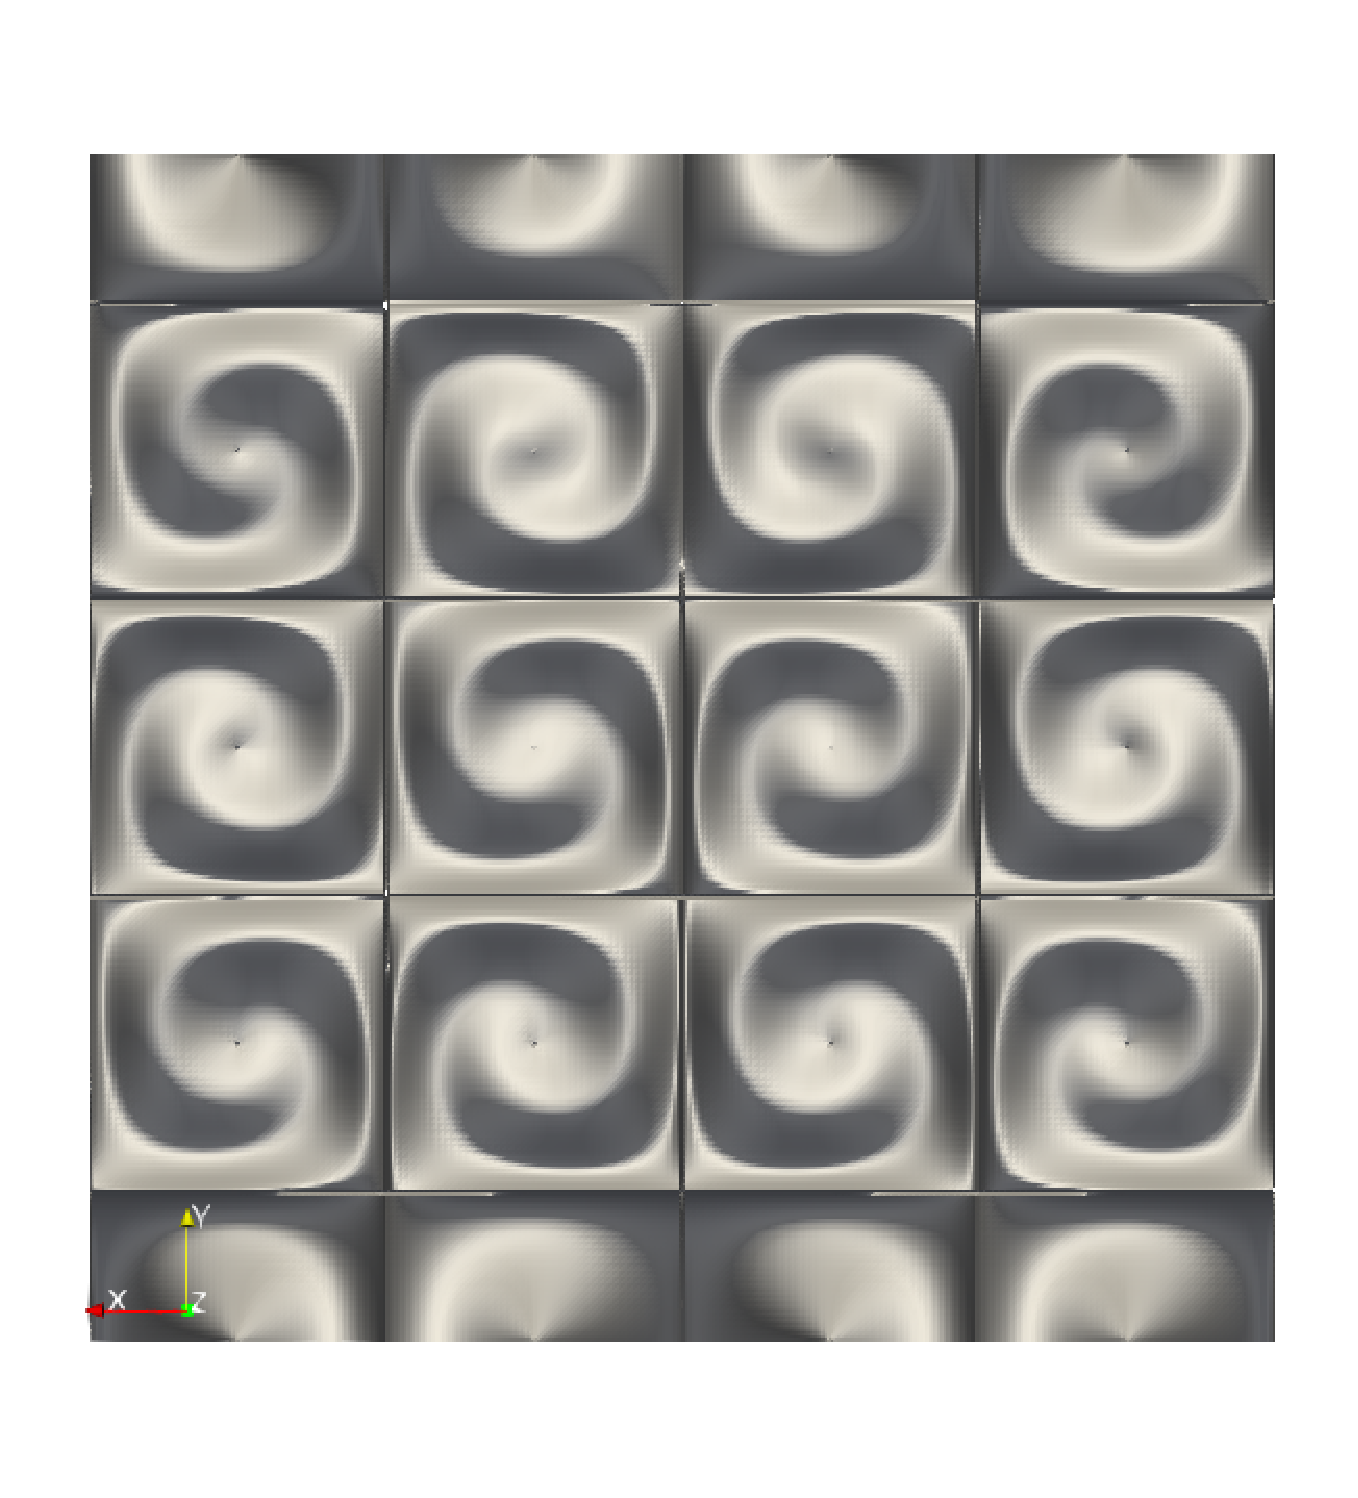
\includegraphics[height=1.1in,width=1.1in,angle=0]{scenes/scene_80.pdf}}
\subfigure[]{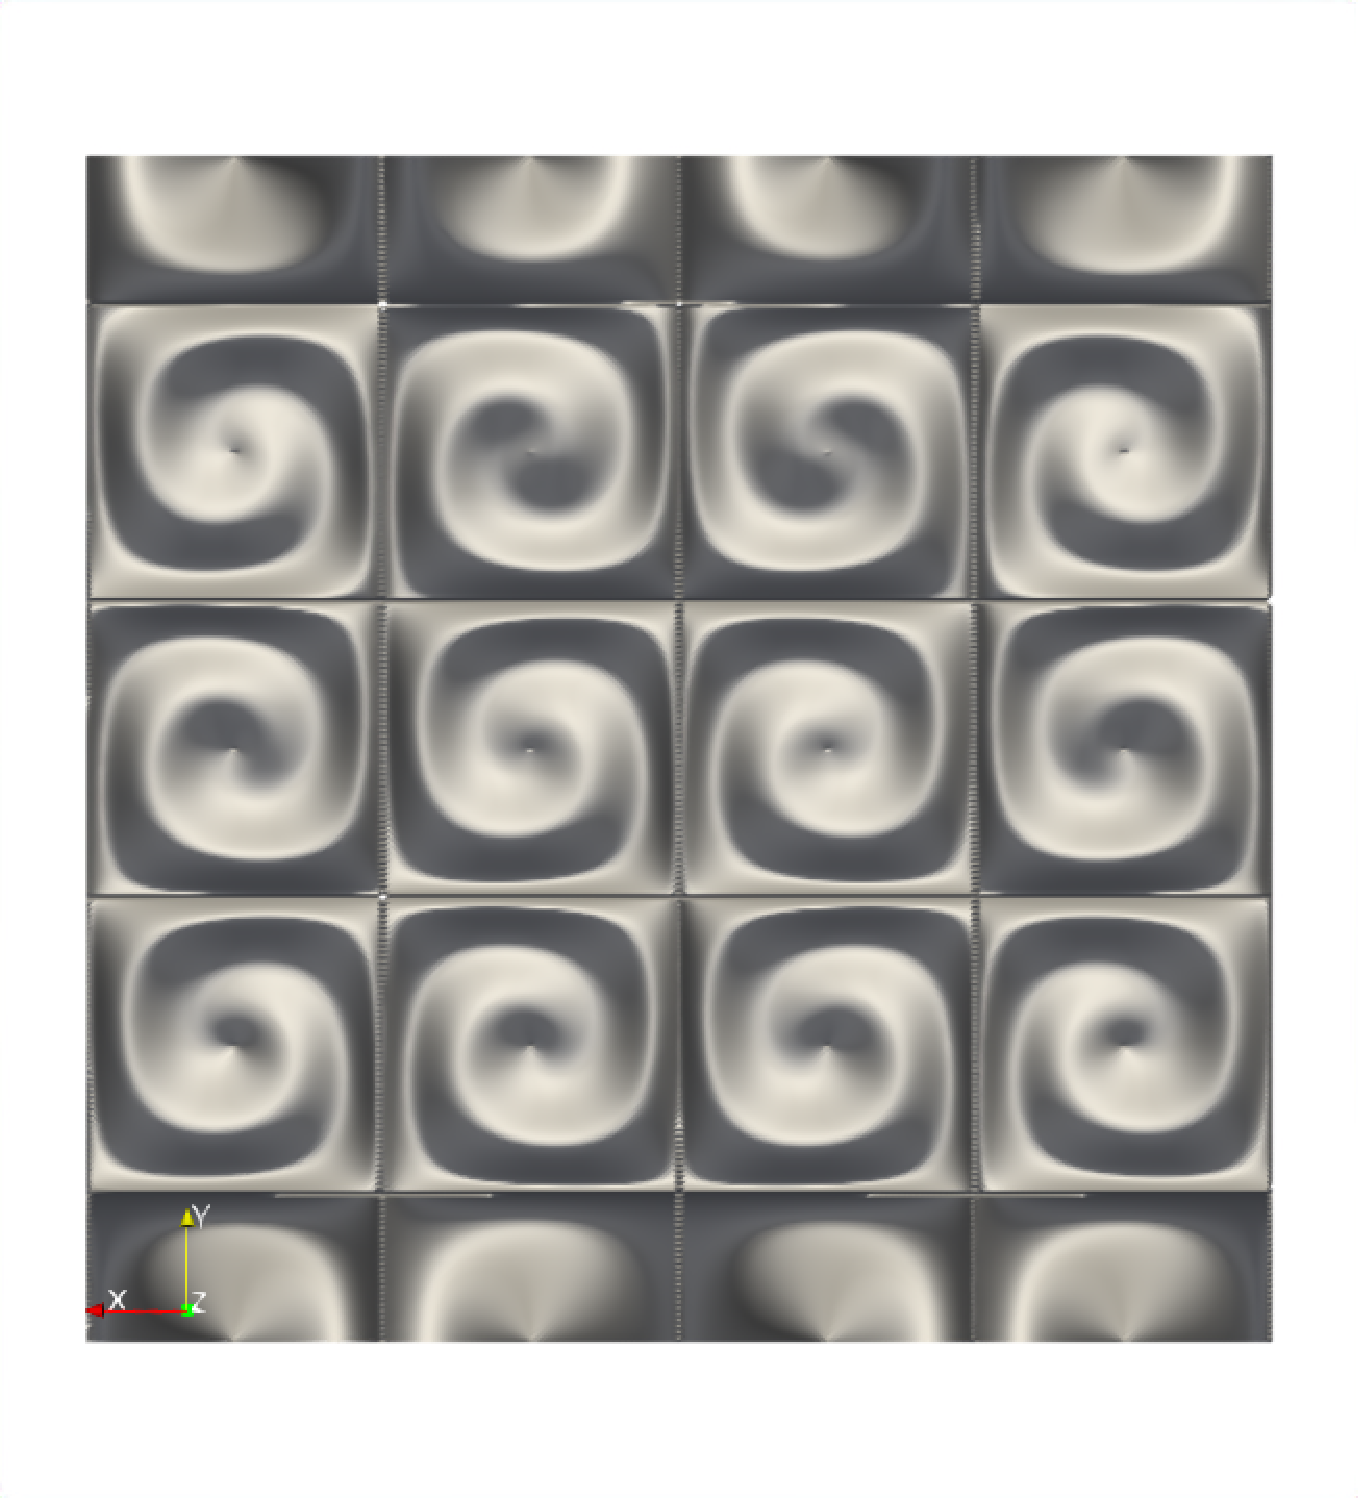
\includegraphics[height=1.1in,width=1.1in,angle=0]{scenes/scene_100.pdf}}
\caption{Variation of the surface at the iterations (a) 0 (b) 20 (c) 40 (d) 60 (e) 80 (f) 100}
\end{center}
\end{figure}
\pagebreak
Secondly we selected Z values as the empty Z column in our output files then we used "Delaunay2D" and we used "Contour" to contour the surface with the Q values. We set 100 ishoypes between double the maximum and minimum Q values of the initial condition output. The gradual change of the crossings of the surface with the isohypes can be seen as shown in the Figure 3.2.
\begin{figure}
\begin{center}
\subfigure[]{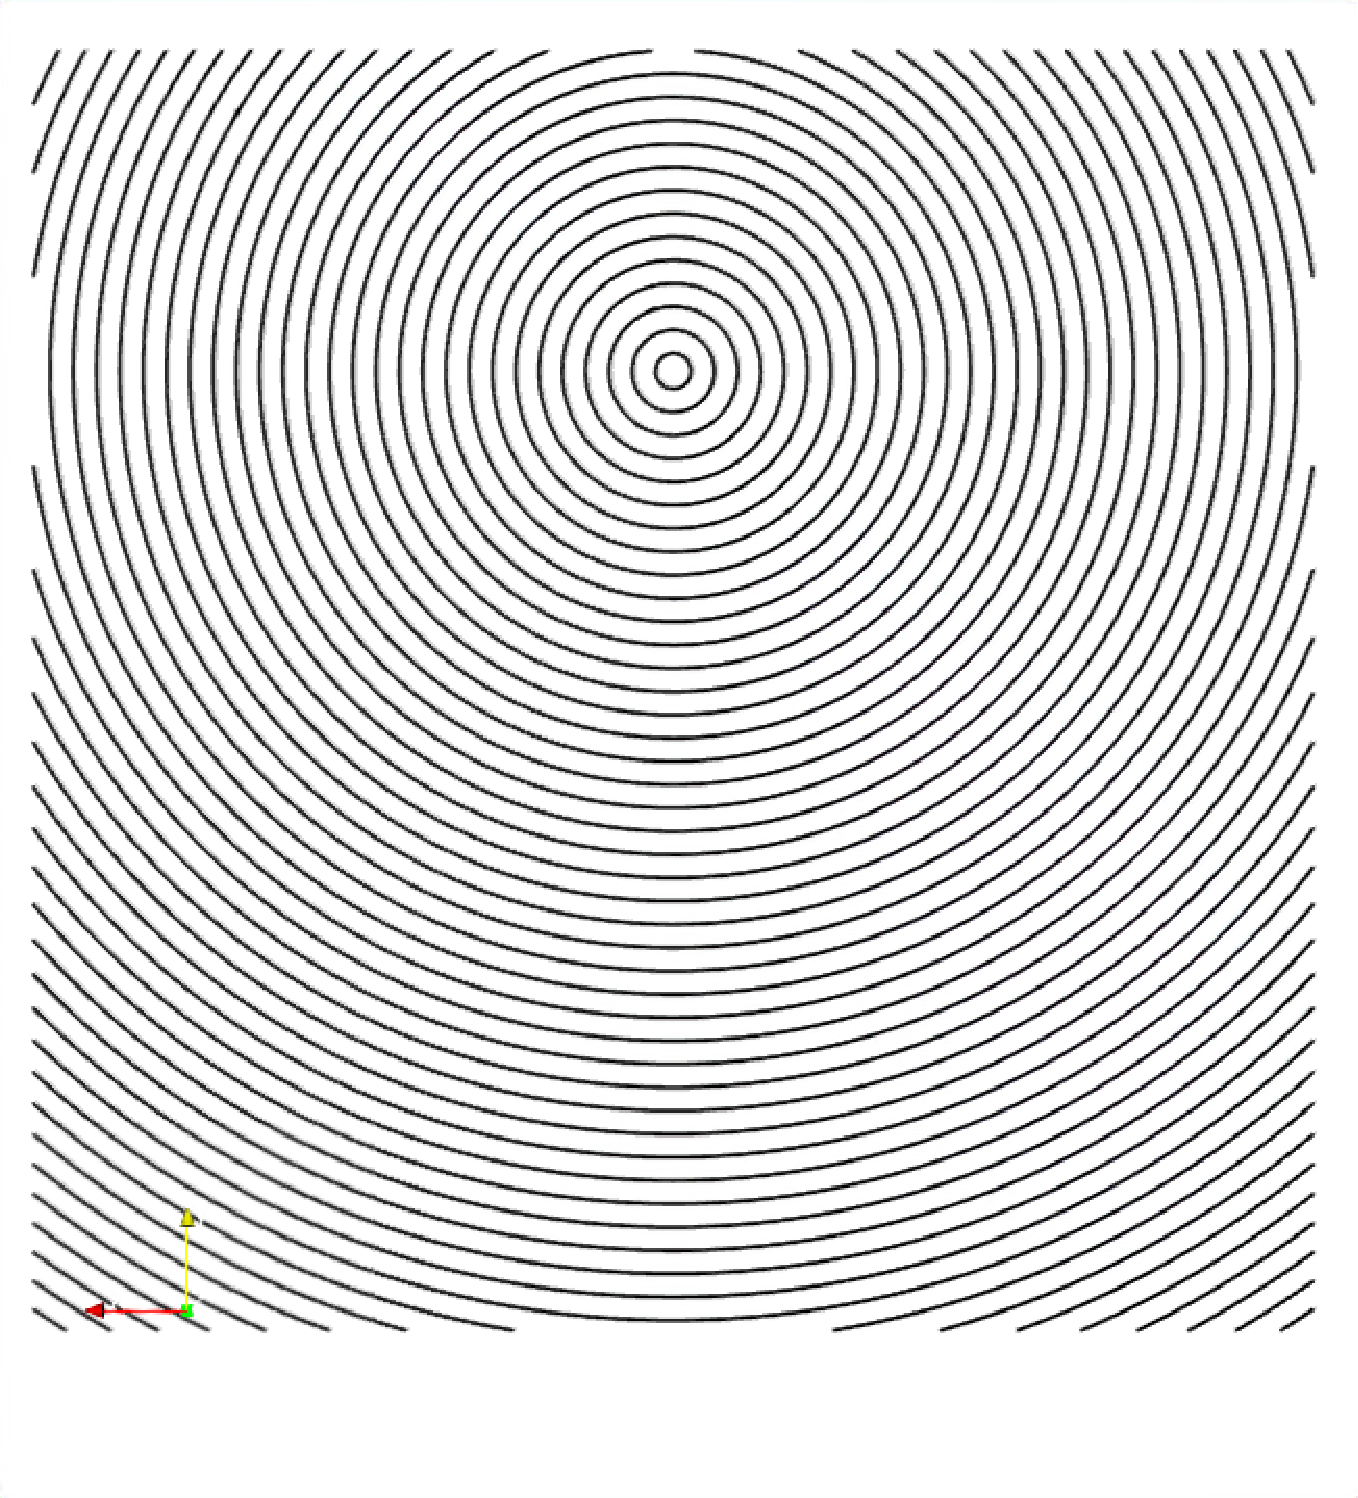
\includegraphics[height=1.2in,width=1.2in,angle=0]{countours/countour_0.pdf}}
\subfigure[]{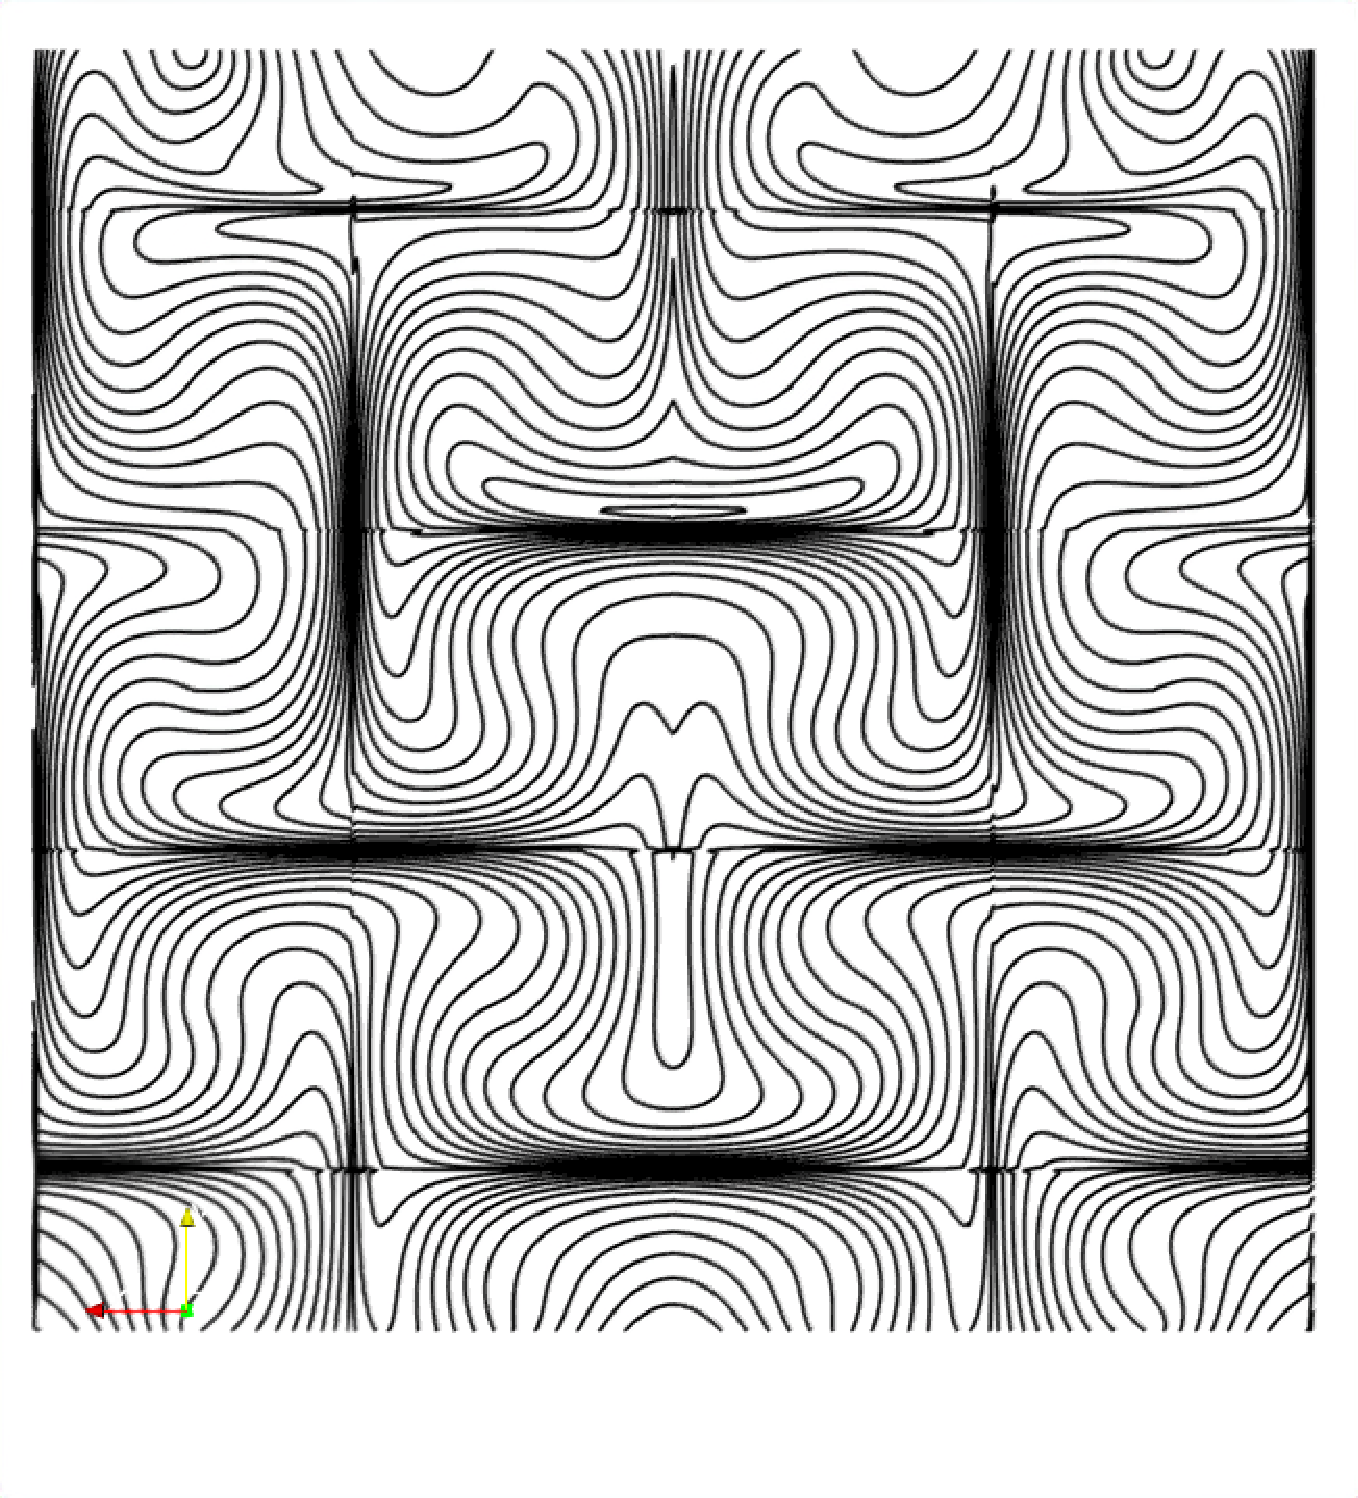
\includegraphics[height=1.2in,width=1.2in,angle=0]{countours/countour_20.pdf}}
\subfigure[]{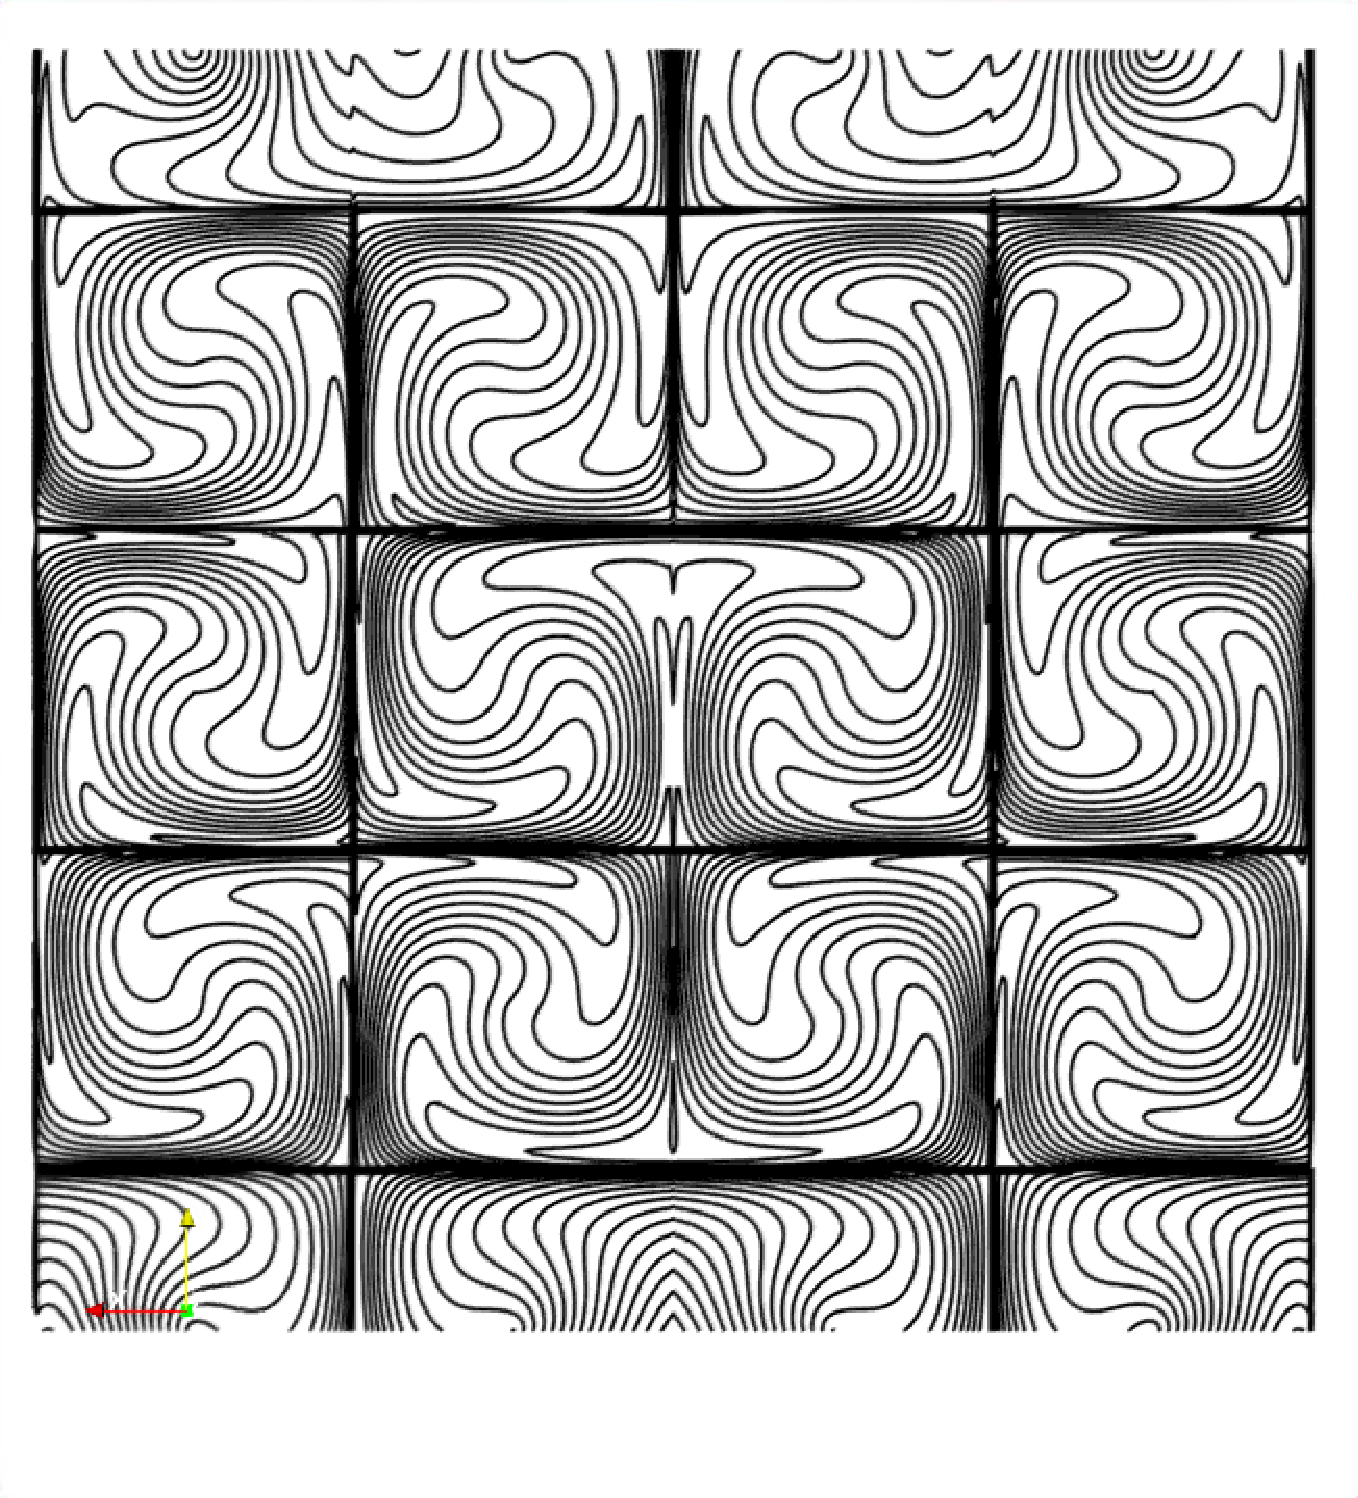
\includegraphics[height=1.2in,width=1.2in,angle=0]{countours/countour_40.pdf}}
\subfigure[]{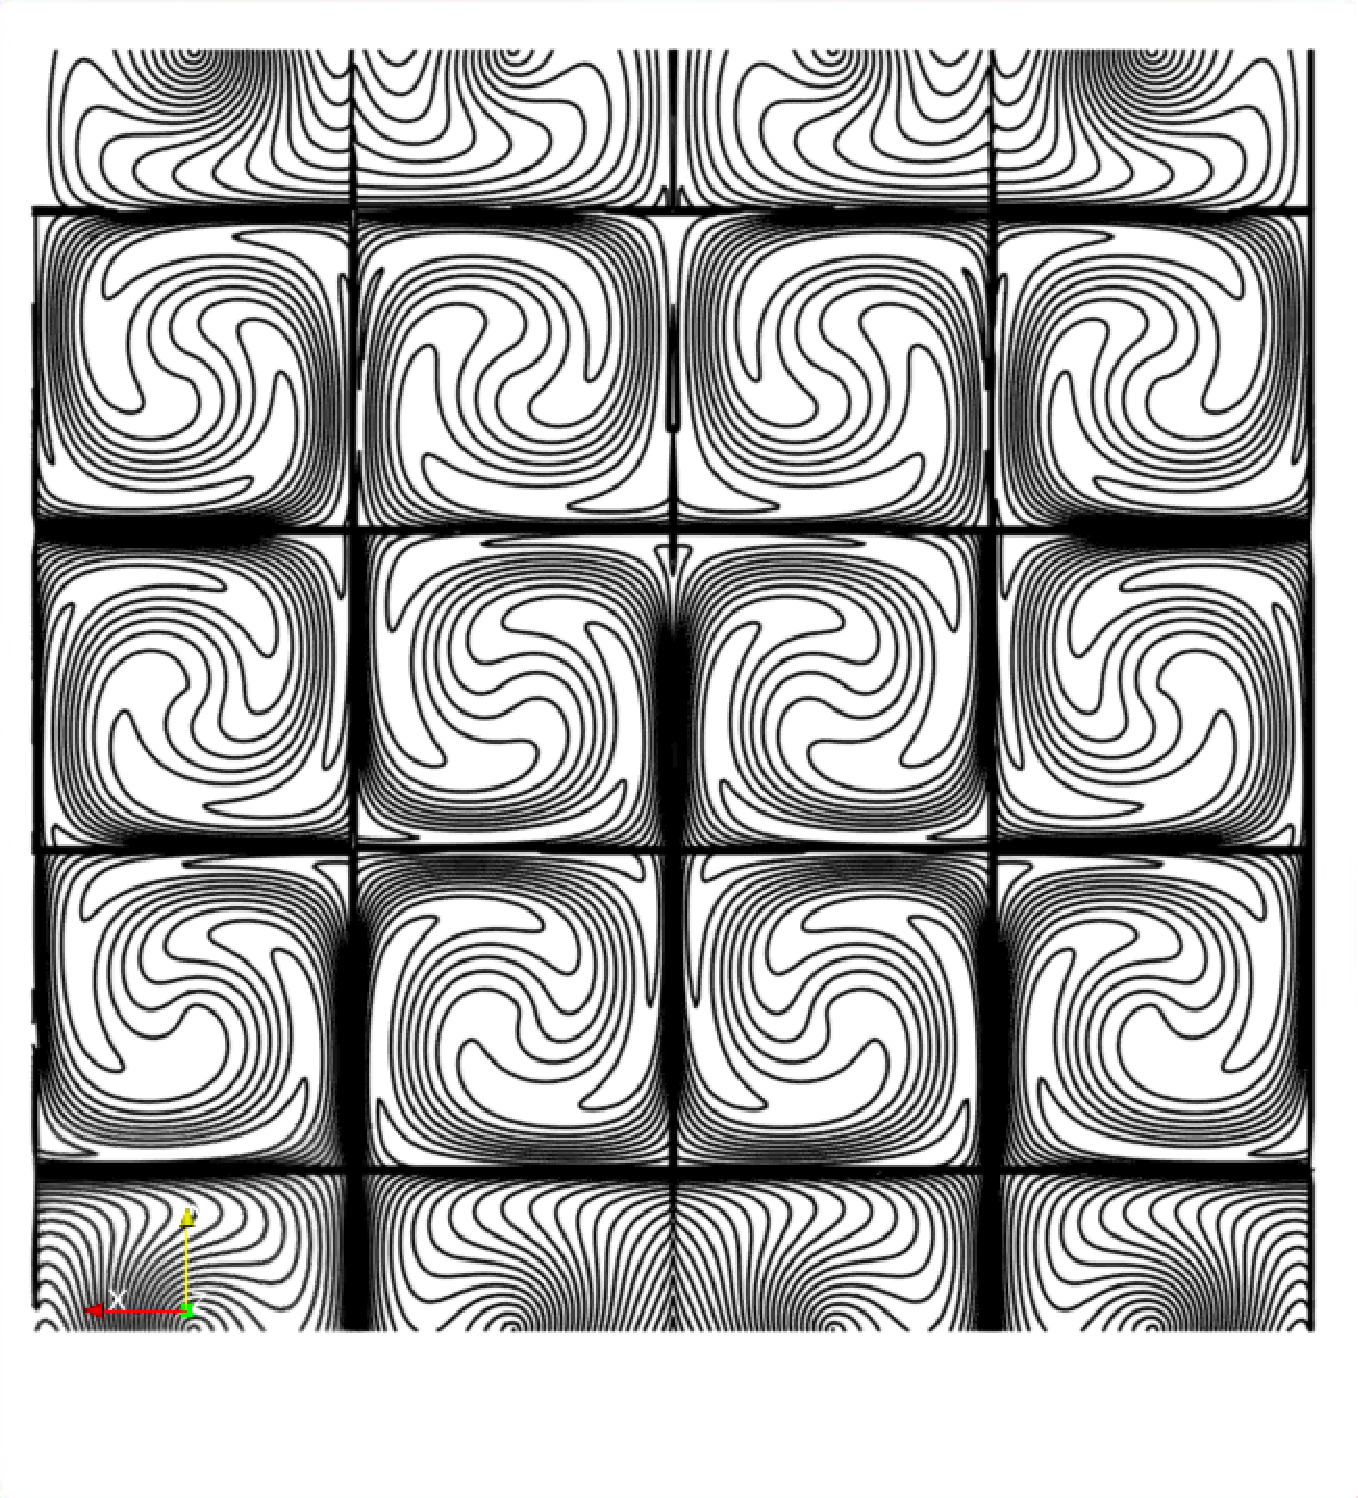
\includegraphics[height=1.2in,width=1.2in,angle=0]{countours/countour_60.pdf}}
\subfigure[]{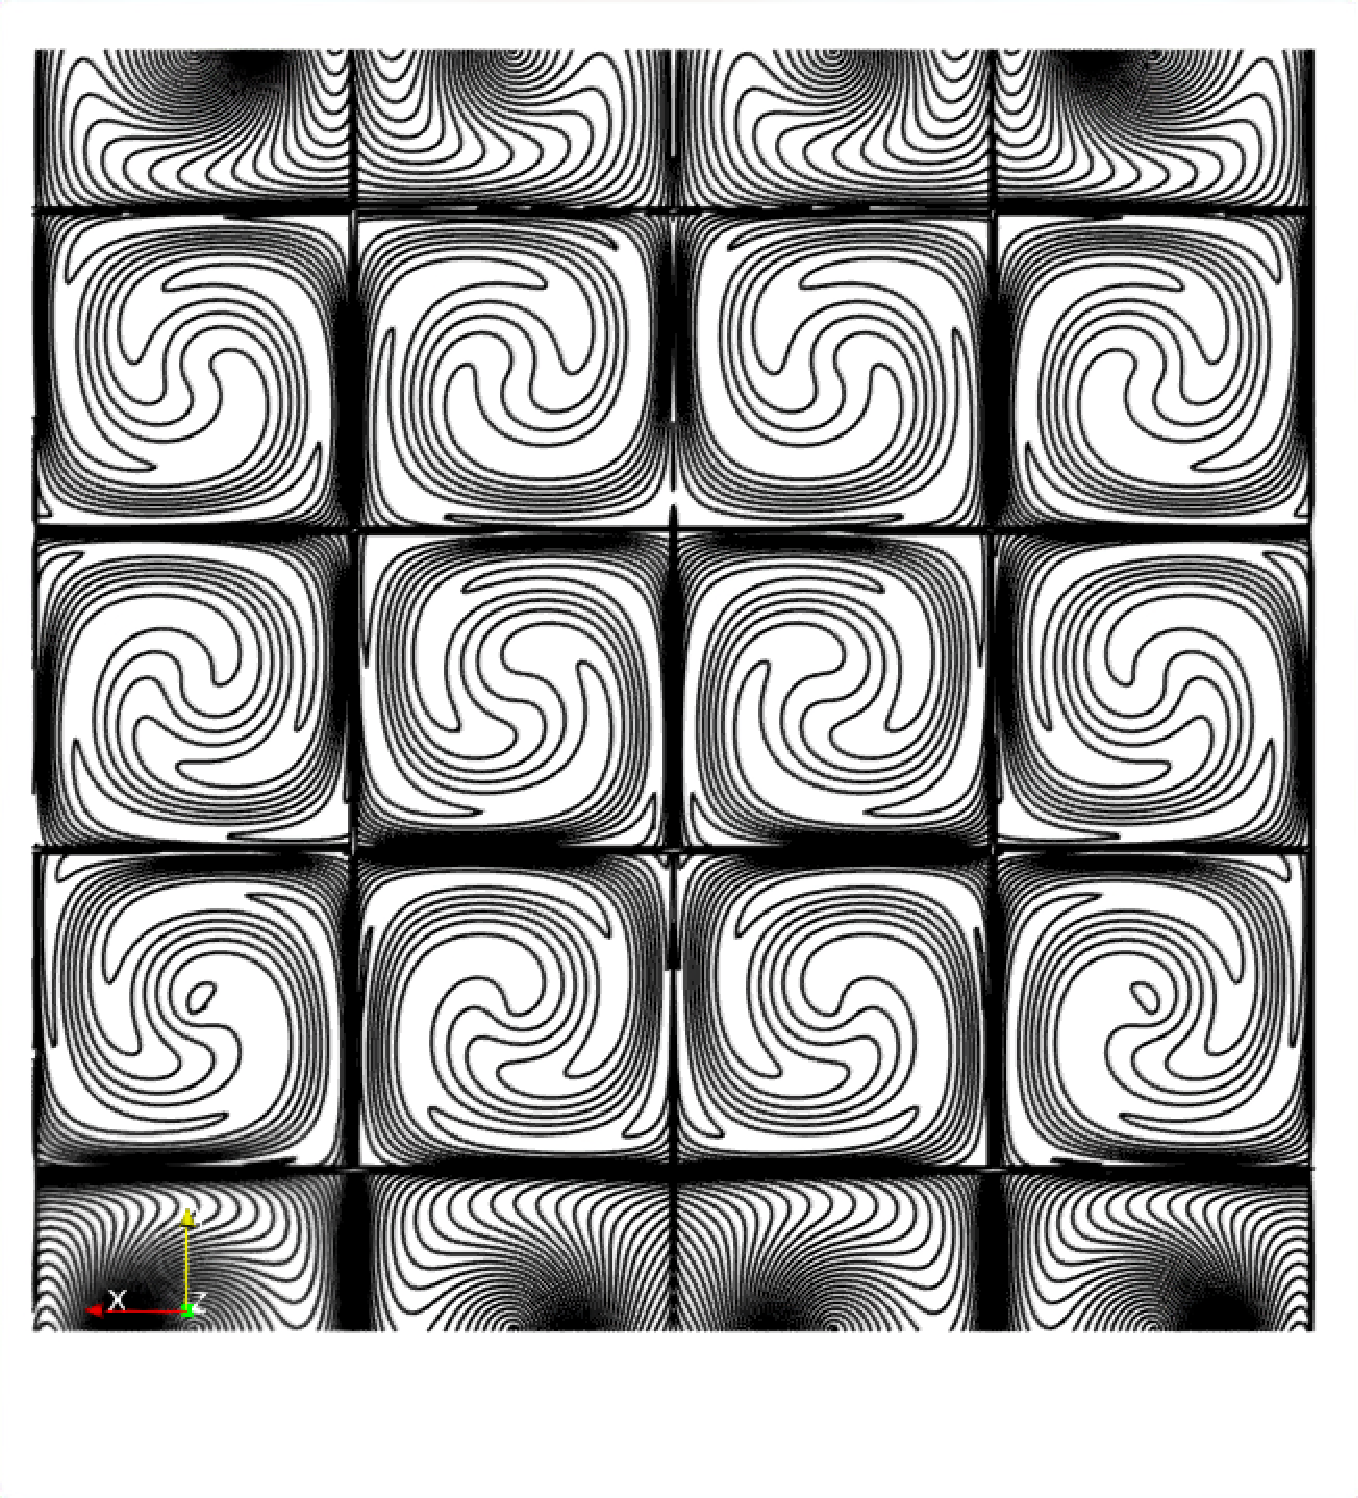
\includegraphics[height=1.2in,width=1.2in,angle=0]{countours/countour_80.pdf}}
\subfigure[]{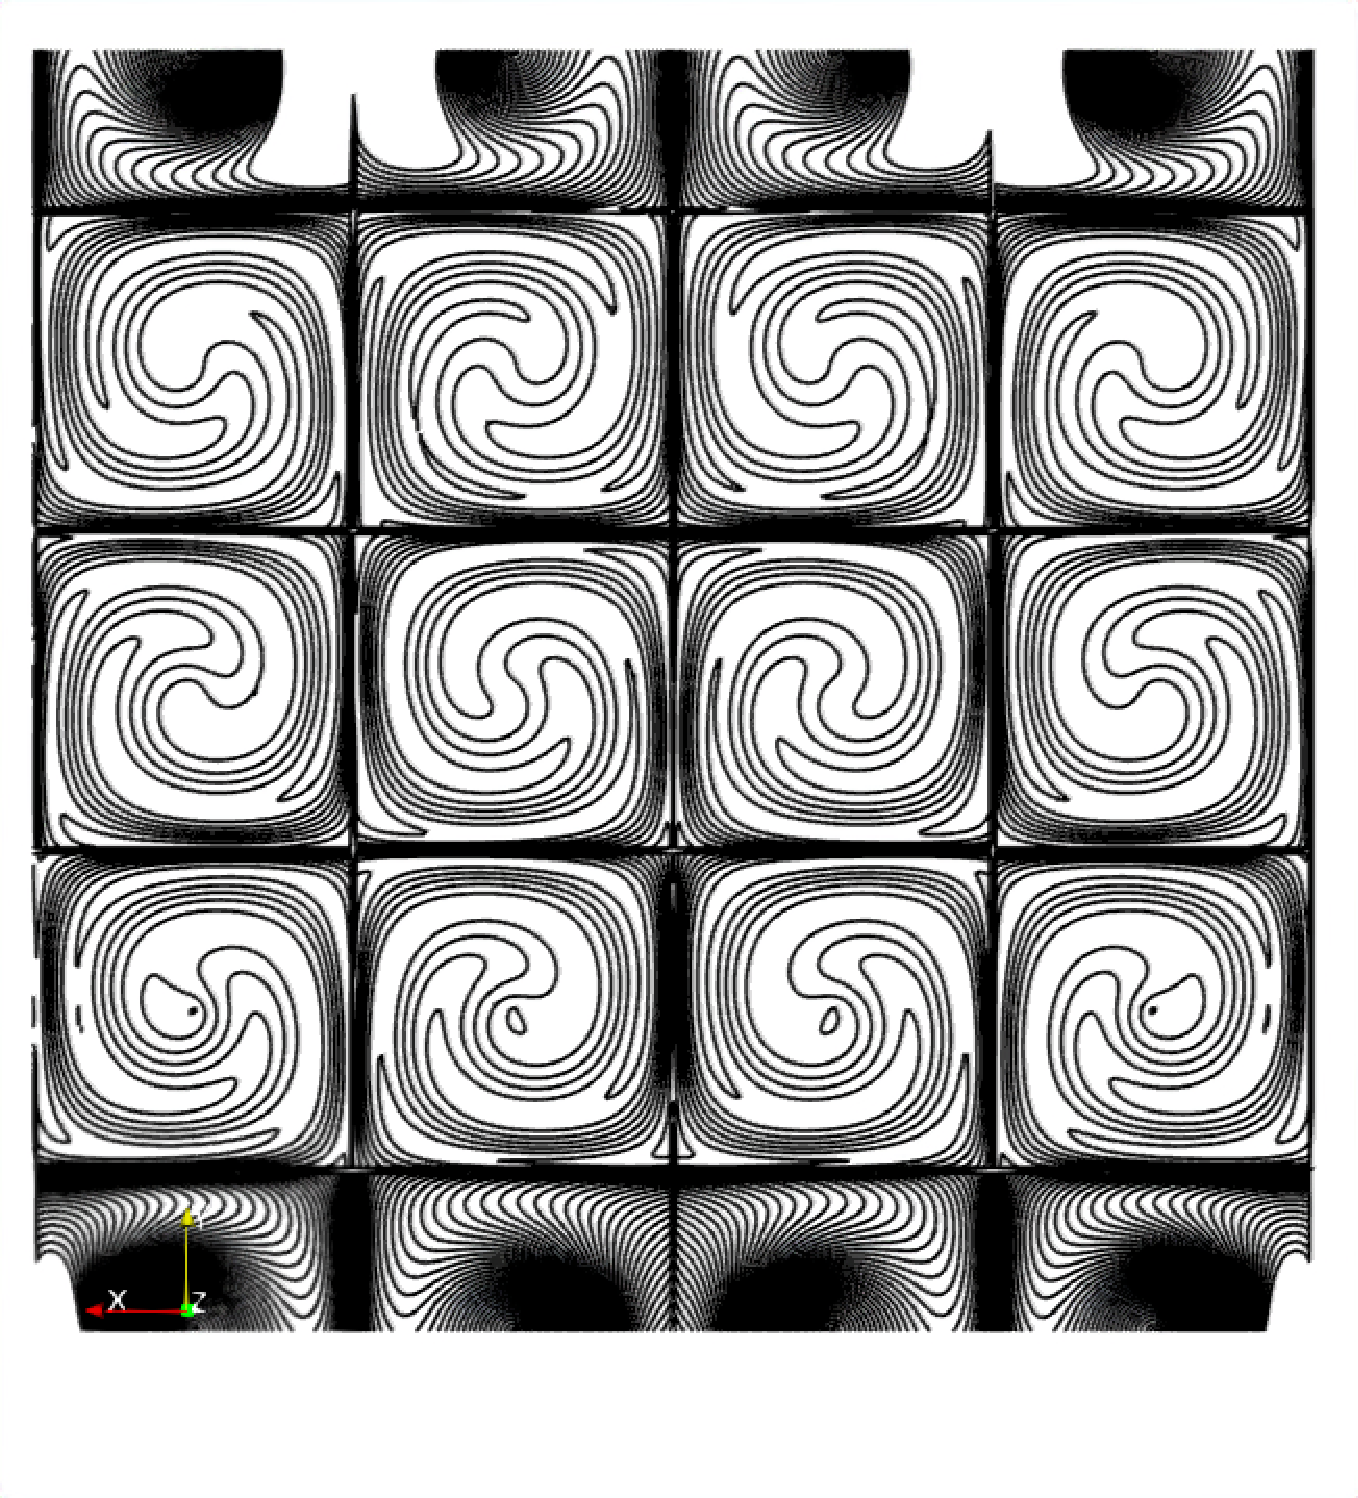
\includegraphics[height=1.2in,width=1.2in,angle=0]{countours/countour_100_r.pdf}}
\caption{Variation of isohypes crossings at the iterations (a) 0 (b) 20 (c) 40 (d) 60 (e) 80 (f) 100}
\end{center}
\end{figure}
\pagebreak
Because we preserved the same isohypes for all of the iterations it looks like some empty space is forming on the top of our surface from the isohypes. But we know that is not the case as we see the contrary from the Figure 3.1. Hence we are forming new isohypes in order to reflect our solution. The 100th iteration can be seen in the Figure 3.3.
\begin{figure}
    \centering
    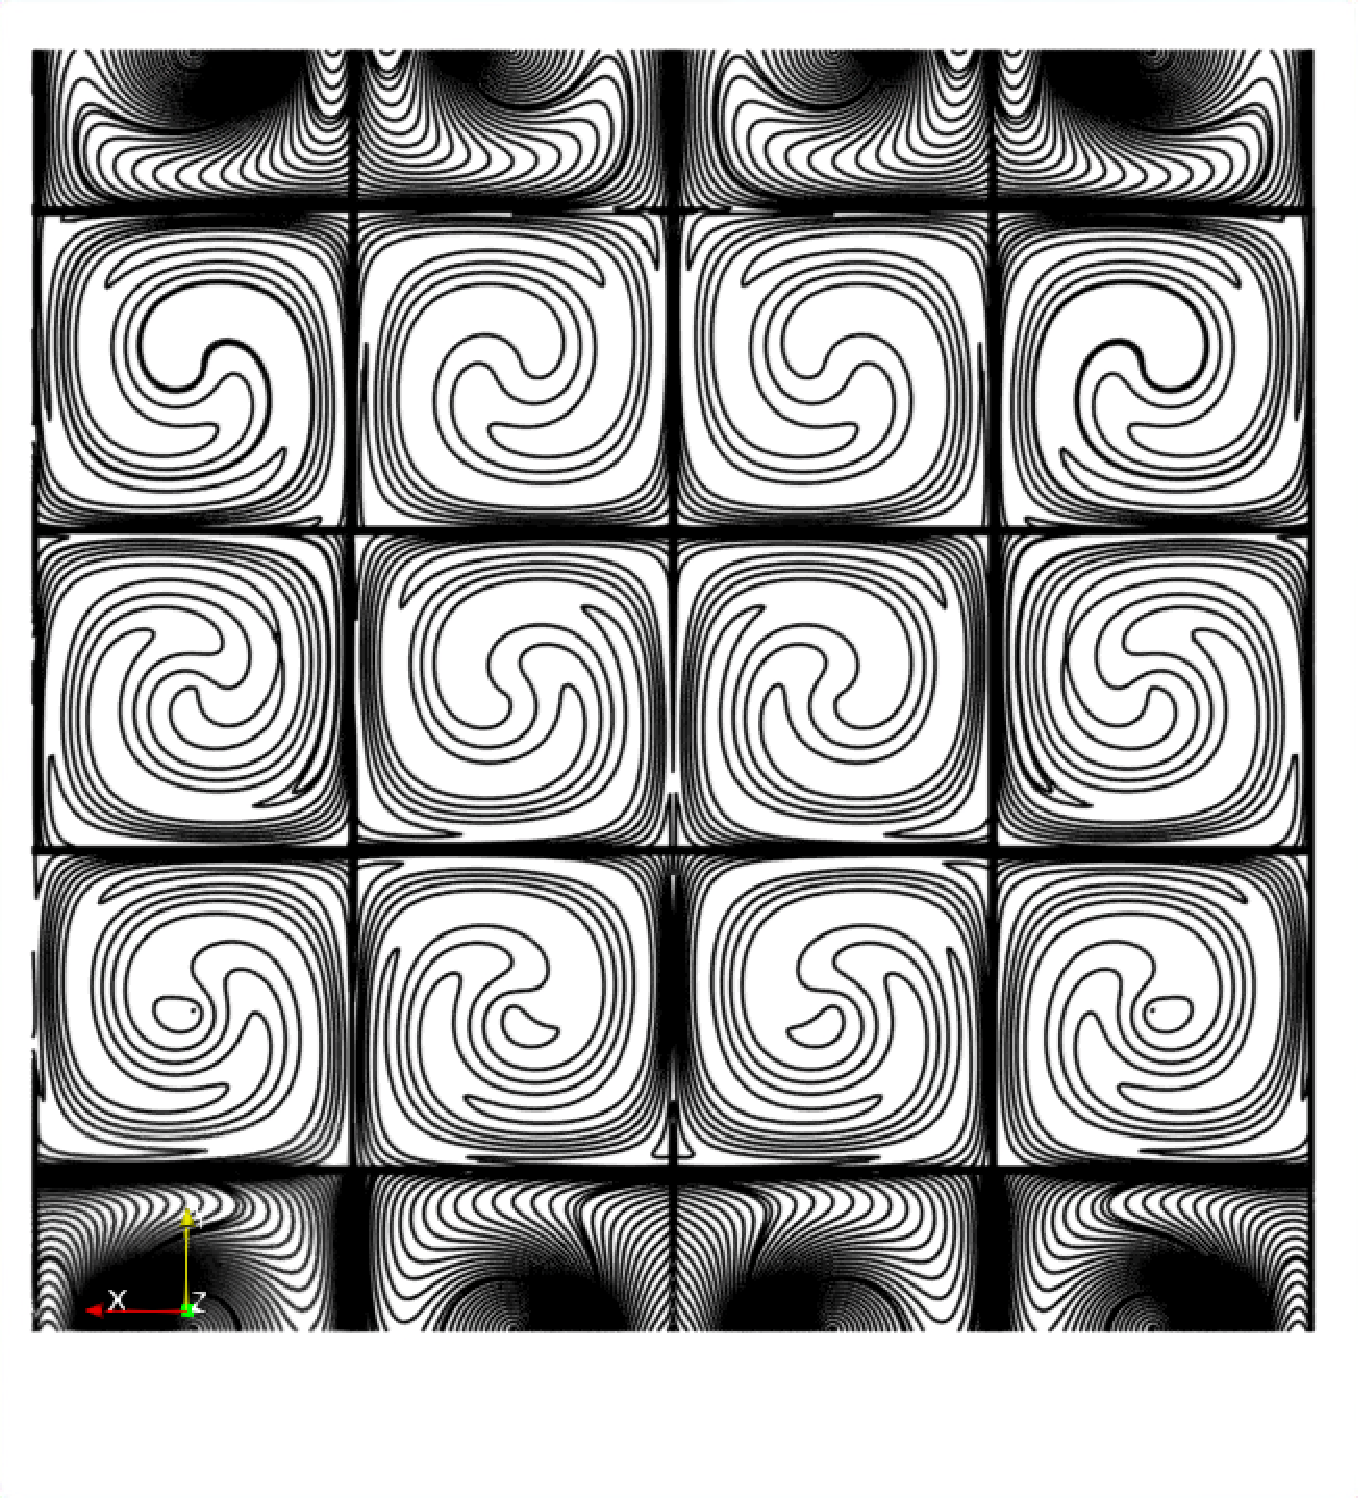
\includegraphics[height=3in,width=3in,angle=0]{countours/countour_100.pdf}
    \caption{End result}
\end{figure}






\end{document}
